\subsection{Curva de calibración}

Los datos obtenidos de densidad óptica desde una muestra con número de células viables de detalla en la tabla \ref{tab:cal_brut}

\begin{table}[H]
  \centering
  \begin{tabular}{ccccccccc}\toprule
    & \multicolumn{7}{c}{Dilución en relación a muestra original} & \\ \cmidrule{2-8}
    & 1:2 & 1:4 & 1:8 & 1:16 & 1:32 & 1:64 & 1:128 & Blanco \\ \cmidrule{2-9}
    & 0.905 & 0.537 & 0.307 & 0.183 & 0.110 & 0.077 & 0.061 & 0.044 \\
    & 0.905 & 0.537 & 0.303 & 0.178 & 0.111 & 0.077 & 0.059 & 0.042 \\
    & 0.918 & 0.542 & 0.310 & 0.180 & 0.113 & 0.077 & 0.061 & 0.041 \\ \midrule
    Promedio & 0.909 & 0.539 & 0.307 & 0.180 & 0.111 & 0.077 & 0.060 & 0.042 \\ \bottomrule
  \end{tabular}
  \caption{Densidad óptica muestras con \si{\ufc\per\mL} conocida (datos en bruto)}
  \label{tab:cal_brut}
\end{table}


Se ajustaron los datos para obtener la densidad óptica de la muestra, ya que la presentada en la tabla \ref{tab:cal_brut} indica la densidad óptica tanto del organismo como del medio de cultivo, lo que son presentado en la tabla \ref{tab:cal_adj}

\begin{table}[H]
  \centering
  \begin{tabular}{cccccccc}\toprule
    & \multicolumn{7}{c}{Dilución en relación a muestra original} \\ \cmidrule{2-8}
    & 1:2 & 1:4 & 1:8 & 1:16 & 1:32 & 1:64 & 1:128 \\ \cmidrule{2-8}
    & 0.861 & 0.493 & 0.263 & 0.139 & 0.066 & 0.033 & 0.017 \\
    & 0.863 & 0.495 & 0.261 & 0.136 & 0.069 & 0.035 & 0.017 \\
    & 0.877 & 0.501 & 0.269 & 0.139 & 0.072 & 0.036 & 0.02 \\ \midrule
    Promedio & 0.867 & 0.496 & 0.264 & 0.138 & 0.069 & 0.035 & 0.018 \\ \bottomrule
  \end{tabular}
  \caption{Densidad óptica muestras con \si{\ufc\per\mL} conocida (datos corregidos)}
  \label{tab:cal_adj}
\end{table}

Dado que el inocuo inicial contenía \SI{4.5e9}{\ufc\per\mL}, los títulos de las diluciones seriadas están totalmente determinado y se adjuntan en la siguiente tabla

\begin{table}[H]
  \centering
  \begin{tabular}{cc}\toprule
    Dilución & Título ($\times$\SI{e9}{\ufc\per\mL}) \\ \midrule
    1:2 & 2.25 \\
    1:4 & 1.12 \\
    1:8 & 0.562 \\
    1:16 & 0.281 \\
    1:32 & 0.141 \\
    1:64 & 0.0704 \\
    1:128 & 0.0352 \\ \bottomrule
  \end{tabular}
  \caption{Título diluciones}
  \label{tab:tab_title}
\end{table}

Entonces, a partir de los datos experimentales detallados previamente, es que se construyó una \emph{curva de calibración} que relaciona la densidad óptica (DO) medida con la cantidad de células viables (\si{\ufc\per\mL}), la que ilustra en la figura \ref{fig:cal_curve}

\begin{figure}[H]
  \centering
  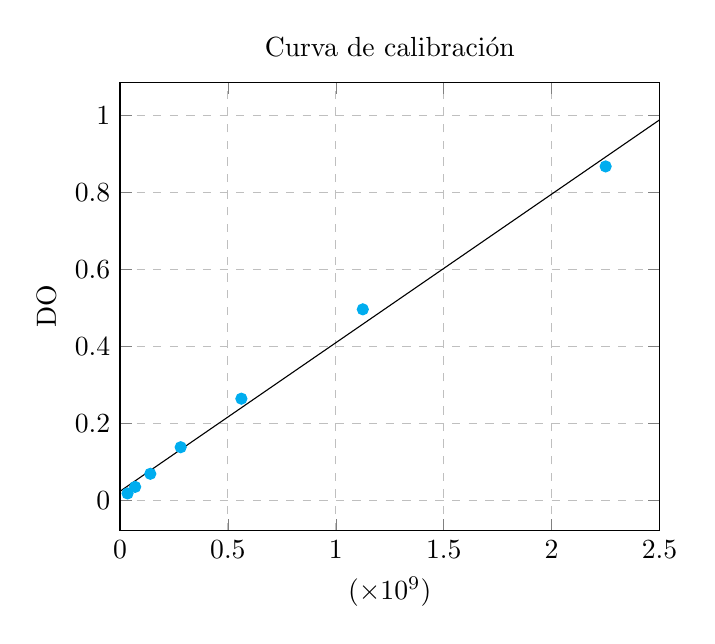
\begin{tikzpicture}[baseline=(current bounding box.center)]
    \begin{axis}[
        title={Curva de calibración}, 
        xlabel={\si{\ufc\per\mL}($\times10^9$)},
        ylabel={DO},
        xmin=0, xmax=2.5,
        xticklabel style={ 
          /pgf/number format/precision=3, 
          /pgf/number format/fixed}, 
        legend pos = north west, 
        ymajorgrids=true, 
        xmajorgrids=true, 
        yminorgrids=true, 
        xminorgrids=true, 
        grid style=dashed]

      \addplot[only marks, color=cyan]
        coordinates {
          (2.25, 0.867)
          (1.125, 0.496)
          (0.5625, 0.264)
          (0.28125, 0.138)
          (0.140625, 0.069)
          (0.0703125, 0.035)
          (0.03515625, 0.018)
        };

      \addplot[no marks] {0.385792*x+0.0235};

    \end{axis}
  \end{tikzpicture}
  \caption{Curva de calibración}
  \label{fig:cal_curve}
\end{figure}
